\section{Ciclo de Vida de los archivos}

Antes de ver los comandos más básicos de git, debemos de conocer el ciclo de vida de los archivos que estos pueden tener cuando se trabajan con \emph{git}.
Estas de dividen en 4 etapas:
\begin{enumerate}
	\item \textbf{Untracked: } Esto significa que Git no está siguiendo el archivo. Es decir, Git no sabe acerca de los cambios en este archivo y no lo incluirá en tu próximo commit a menos que lo agregues explícitamente con git add. Los archivos suelen estar en este estado cuando son nuevos en el repositorio.
	\item \textbf{Unmodified: } Un archivo se encuentra en este estado cuando está en el repositorio y no ha sido modificado desde la última confirmación (commit). Git está al tanto de este archivo y no se realizaron cambios en él desde la última confirmación.
	\item \textbf{Modified: } Después de modificar un archivo que Git está rastreando, el estado de ese archivo cambia a "Modificado". Esto significa que han habido cambios en el archivo desde la última confirmación y Git los ha detectado, pero aún no se han preparado para una nueva confirmación.
	\item \textbf{Staged: } Cuando decides que quieres incluir los cambios de un archivo modificado en tu próxima confirmación, lo añades al área de preparación (staging area) con git add. Una vez que un archivo está en el área de preparación, se considera "preparado" y está listo para ser confirmado en el repositorio.
\end{enumerate}

\begin{figure}[h!]
		\centering
		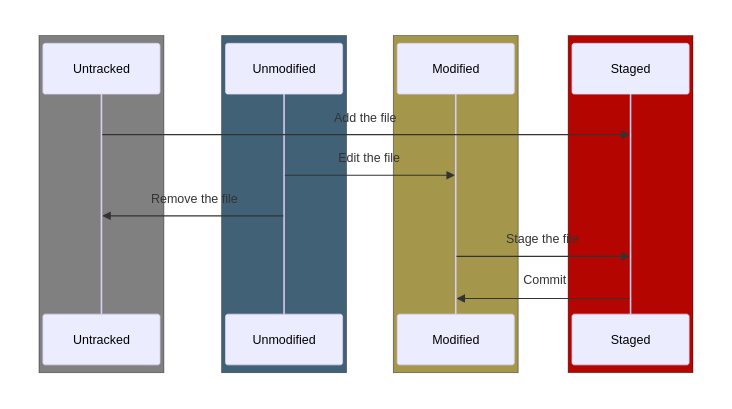
\includegraphics[width=0.85\textwidth]{04FundamentosDeGit/Imagenes/cicloDeVida00.png}
		\caption{Ciclo de vida los archivo en Git}
		\label{fig:cicloDeVida}
\end{figure}

\newpage

\section{Fundamentos De Git}

Durante el siguiente capítulo, vamos a conocer los comandos básicos de Git, con los cuales vamos a poder:

\begin{itemize}
	\item Inicializar un repositorios
	\item Verificar el seguimiento de archivos
	\item Commit
	\item Ignorar archivos no deseados
	\item Errores comunes
	\item Navegar por el historial de nuestro proyecto
\end{itemize}

\begin{pucpImportant}
Para conocer más información sobre los diversos comandos que existen en git, y puede revisarla con algunos de los siguiente comandos:

	\begin{gitCode}
		\mint{bash}|git help <comando> # Recomendado si trabaja desde Windows|
		\mint{bash}|git <comando> --help|
		\mint{bash}|man git <comando>  # Recomendado si trabaja desde Linux|	
	\end{gitCode}

Ejemplo de uso:

	\begin{terminal}
		\mint{bash}|git help config|
		\mint{bash}|git config --help|
		\mint{bash}|man git config|
	\end{terminal}

\end{pucpImportant}

\subsection{Inicializar un respositorio de Git}

Para iniciar un nuevo proyecto, nos vamos a dirigir al directorio de nuestro y vamos a abrir nuestra terminal.

\begin{gitCode}
\begin{minted}{bash}
git init 
\end{minted}
\end{gitCode}

Con este comando se nos va a crear un carpeta \textit{\textbf{.git}}  dentro de nuestro proyecto, el cuál va a contener los archivo necesarios para el repositorio.

\subsection{Estado de los archivos}

La herramienta para poder conocer el estados de cualquier archivo, es con el siguiente comando:

\begin{gitCode}
\begin{minted}{bash}
git status # Para ver la informacion de todos los archivos
git status nombre-del-archivo # Para ver informacion de un único archivo
\end{minted}
\end{gitCode}

Ejemplo con la creación de un archivo, por ejemplo si vamos a agregar un \emph{README.md} al proyecto.

\begin{terminal}
\begin{minted}{bash}
#===================================================
# Codigo
#===================================================
echo 'Nombre-del-proyecto' >> README.md
git status
#===================================================
#Output
#===================================================
On branch main

No commits yet

Untracked files:
(use "git add <file>..." to include in what will be committed)
README.md

nothing added to commit but untracked files present (use "git add" to track)
\end{minted}
\end{terminal}

Como nos podemos percatar, no solo nos da información sobre los archivos, sino también sobre la rama en la que estamos trabajando; el
manejo de las ramificaciones en \emph{git} se realizará más adelante.

Así mismo, si solo queremos conocer la información de los archivos, de una manera más corta, se puede hacer uso del siguiente comando:

\begin{gitCode}
\begin{minted}{bash}
#===================================================
# Codigo
#===================================================
git status -s # -s es abreviatura de --short
#===================================================
# Output
#===================================================
?? README.md
#===================================================
# Forma general
#===================================================
XY nombre-del-archivo
\end{minted}
\end{gitCode}

Los valores de XY, va a depender de los cambios que haigamos realizados, estos pueden tener 8 posibles valores:

\begin{multicols}{2}
	\begin{enumerate}
		\item \textbf{` ':} sin modificar
		\item \textbf{M :} modificado
		\item \textbf{T :} Tipo de archivo modificado
		\item \textbf{A :} añadido
		\columnbreak
		\item \textbf{D : } borrado
		\item \textbf{R : } renombrado
		\item \textbf{C :} copiado
		\item \textbf{U :} actualizado pero no fusionado
	\end{enumerate}
\end{multicols}

Para ver una lista de cada uno de las posibles combinaciones y su significado, puede revisar la \href{https://git-scm.com/docs/git-status}{\textcolor{pucpRojo}{documentación}}
o revisar la documentación de git status como se explico anteriormente.

\subsection{Rastreo de los archivos}

Los archivos rastreados son aquellos que ya pertenecen al proyecto, estos pueden ser modificados, sin modificar o preparados. Los archivos sin rastrear son todos los demás.

Para empezar a rastrear un archivo, vamos a ejecutar el siguiente comando:

\begin{gitCode}
\begin{minted}{bash}
git add . # Todos los archivos, incluso los que ya estaban rastreados
git add NombreDelArchivo # Solo el archivo indicado
\end{minted}
\end{gitCode}

\begin{pucpImportant}
	Si vamos a agregar multiples archivos, directorios o demás, ir escribiendo 1 por 1 puede ser muy tardado, por lo que se recomienda usar
\href{https://berkeley-scf.github.io/tutorial-using-bash/regex.html}{\textcolor{pucpRojo}{expresiones regulares}}.
\end{pucpImportant}

\subsection{Ignorar archivos}

Esta opción puede parecer algo raro, ya que normalmente pensamos que todos los archivos 
que tengamos en nuestro proyecto son esenciales, pero no siempre es así. Ejemplo:

\begin{itemize}
	\item La carpeta \textit{.vscode}, la cual contiene información de como nosotros personalizamos nuestro entorno de trabajo en \textbf{vscode}, la cual no es relevante para el proyecto.
	\item Archivos generados al momento de compilar un proyecto, esos archivos siempre se generan cuando se compila; por lo tanto, no es necesario incluirlo.
\end{itemize}














